\documentclass[tikz,border=10pt]{standalone}
\usepackage{tikz}
\usetikzlibrary{arrows.meta,patterns,positioning}

\begin{document}
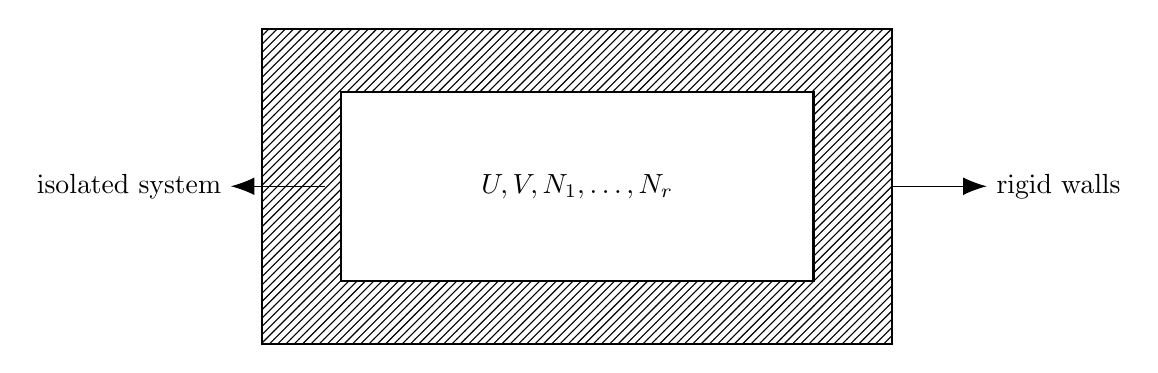
\begin{tikzpicture}
    % Outer rigid walls
    \draw[thick,pattern=north east lines] (-4,-2) rectangle (4,2);
    % Inner system box
    \draw[thick,fill=white] (-3,-1.2) rectangle (3,1.2);
    \node at (0,0) {$U, V, N_1,\ldots,N_r$};

    % Labels
    \draw[-{Latex[length=3mm]}] (-3.2,0) -- (-4.4,0) node[left] {isolated system};
    \draw[-{Latex[length=3mm]}] (4,0) -- (5.2,0) node[right] {rigid walls};
\end{tikzpicture}
\end{document}
